\documentclass[tikz,border=10pt]{standalone}
\begin{document}
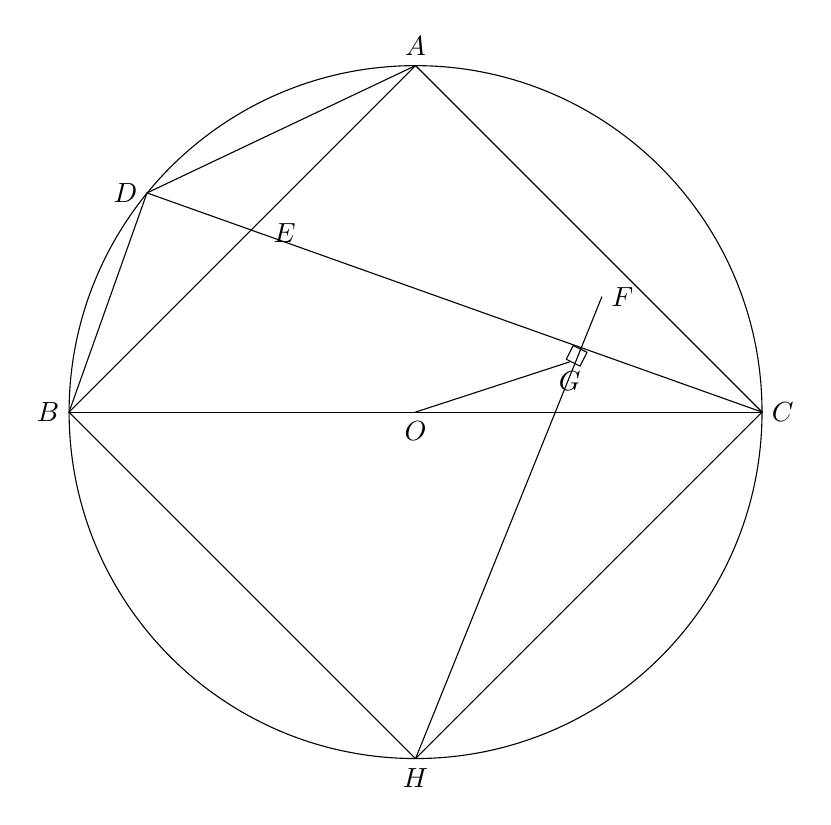
\begin{tikzpicture}[scale=1.1,line cap=round,line join=round]

% Circle and key points
\coordinate (O) at (0,0);
\coordinate (A) at (0,4);
\coordinate (B) at (-4,0);
\coordinate (C) at (4,0);
\coordinate (H) at (0,-4);

% Additional points
\coordinate (D) at (-3.1,2.53);
\coordinate (E) at (-1.75,1.85);
\coordinate (F) at (2.15,1.33);
\coordinate (G) at (1.78,0.58);

% Circle
\draw (-4,0) arc[start angle=180,end angle=540,radius=4];

% Chords and segments
\draw (B) -- (C);
\draw (B) -- (A);
\draw (A) -- (C);
\draw (B) -- (H);
\draw (H) -- (C);

\draw (B) -- (D);
\draw (D) -- (A);
\draw (D) -- (C);

\draw (F) -- (H);
\draw (O) -- (G);

% Right-angle mark at G between DG/GC line and FH line
\draw (1.82,0.77) -- (1.98,0.69) -- (1.90,0.53) -- (1.74,0.61) -- cycle;

% Labels
\node[above] at (A) {$A$};
\node[left] at (B) {$B$};
\node[right] at (C) {$C$};
\node[below] at (H) {$H$};
\node[left] at (D) {$D$};
\node[above right] at (E) {$E$};
\node[right] at (F) {$F$};
\node[below] at (G) {$G$};
\node[below] at (O) {$O$};

\end{tikzpicture}
\end{document}
